\cotefile{77}
\scanpage{82}
que
\[
A_{\Delta}[T]/(T^2+bT+c)
\]
est une extension quadratique étale de $A_{\Delta}$, et sa restriction à $A_{2\Delta}$ est \unsure{isom :|isom. à} $A_{2\Delta}[U]/(U^2-\Delta)$, en posant
\[
U=\frac{1}{2u}\left(T+\frac b2\right).
\]

\deleted{\unsure{Dém}}

\uline{Lemme} \deleted{\unsure{Si} \unsure{vérifie} les conditions \textcircled{a} et \textcircled{b},} \inserted{Supposons $A_{\Delta}$ int. clos dans \deleted{\unsure{\textcircled{d}}} $(A_{\Delta})_{2}$.}
% slanted
\margin{\unsure{dégager|déjà vu|dès que} ceci du \unsure{n\textsuperscript{o}|nb} 2 \uline{\unsure{comme corollaire|comme remarque|connexes}}}

Pour que $\exists\, B_{\Delta}$ ext. quadratique étale de $A_{\Delta}$, se restreignant en $A_{2\Delta}$ suivant $A_{2\Delta}[U]/(U^2-\Delta)$, il \unsure{f. et st|faut et su.} que l'on puisse trouver \inserted{$b,c\in A_{\Delta}$ et} $\unsure{\nu|v}\in\mathbb N$ et \uline{$u\in A_{\Delta}^{*}$} tels que
\[
b^2-4c=\Delta^{\deleted{\unsure{2\nu+1|\nu}}}u^2
\]

Or, quitte \unsure{à|:} multiplier $b,c$ par des puissances \inserted{\unsure{conv.|carr.|carrés}} de $\Delta$, \inserted{($\Delta^\alpha$ et $\Delta^{2\alpha}$ resp\textsuperscript{t})} \unsure{obt\textsuperscript{g}|donc} $b,c\in A$, \deleted{\unsure{Supposons}} \inserted{$u\in A$.}

\deleted{\unsure{alors}} Supposons que \deleted{\unsure{$u$}}
\[
\deleted{\unsure{\text{\textcircled{g}}}}\quad\boxed{\deleted{A_{\Delta}^{*}=\{u\Delta^d\mid d\in\mathbb Z,\ u\in A^*\}}}
\]

\deleted{donc on aura}
\[
\deleted{b^2-4c=\Delta^{2d+1}u^2\qquad(d\in\mathbb Z,\ u\in A^*).}
\]

\deleted{On a $d\in\mathbb N$ \deleted{\unsure{bien}} i.e. $d\geq 0$, car si $d<0$, on aurait}
\[
\deleted{b^2-4c=\Delta^{-\nu}u^2\qquad(\nu>0)}
\]
\deleted{donc}
\[
\deleted{\Delta^\nu(b^2-4c)=u^2}
\]
% archive sheet number: 81
\scanpage{83}
% letterhead

U N I V E R S I T E\\ DES SCIENCES ET TECHNIQUES\\ \uline{DU LANGUEDOC}\\
Montpellier, le 1er décembre 1977\\

JP/MD\\ Diffusion : Liste A\\ n\textsuperscript{o} 6826

AVIS DE SOUTENANCE D'UNE THESE DE DOCTORAT DE SPECIALITE\\ \uline{E C O L O G I E}
% printed form

\uline{Nom et prénom du candidat} : PONT Didier

\uline{Titre de la thèse} : Recherches sur l'évolution saisonnière du peuplement de Copépodes, Cladocènes et Ostracodes des rizières de Camargue.

\uline{Date, heure et lieu de soutenance prévus} : 9 décembre 1977 à 9 h 30, salle de cours n\textsuperscript{o} 10

\uline{Nom du Directeur de thèse} : Monsieur A. CHAMPEAU

\uline{Désignation du laboratoire où la thèse est préparée} : Centre d'écologie de Camargue.

\uline{Analyse de l'ouvrage} : Après avoir mis en évidence les grandes lignes de la structure et de l'évolution saisonnière du peuplement de crustacés des rizières camarguaises sur un grand nombre de stations, l'auteur analyse les résultats obtenus sur 3 stations suivies régulièrement et met en évidence les facteurs de milieu qui conditionnent le fonctionnement du peuplement zooplanctonique.

\uline{Durée approximative des recherches ayant abouti à la thèse} : 2 ans

\uline{Composition du jury proposé} : M. C. SAUVAGE - Président\\ M. AMANIEU\\ M. CHAMPEAU\\ M. DECAMPS\\ M. HEURTEAUX

Le Secrétaire Général,\\
\handwritten{\unsure{E Siau|E Si}}\\
\uline{E. SIAU}

MR LE PROFESSEUR GROTHENDIECK A.\\ MATHEMATIQUES \hfill 5
% archive sheet number: 82
\scanpage{84}

\deleted{d'où $\Delta^{\unsure{\nu|v}}$ \deleted{\unsure{contr.|$A^*$}} $\inserted{\in A^{*}}$ donc $\Delta\in A^*$, et on va supposer}
\[
\deleted{\unsure{\text{\textcircled{h}}}\quad\boxed{\Delta\notin A^*}}
\]

Nous voulons prouver que $u_0$ est él. régulier de $A_0$, \deleted{si $A_0$ est intègre} i.e. qu'il n'est nul en aucune composante irréductible de $A_0$, ce qui résulte de ce qui précède.

\figure{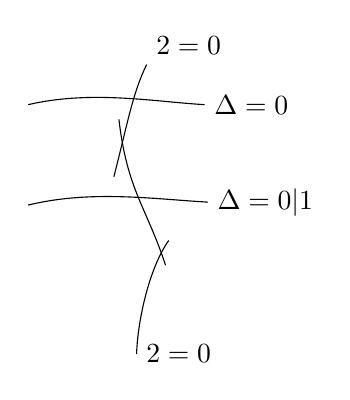
\begin{tikzpicture}[x=.8cm,y=.75cm]\draw (0,3.2) .. controls (1,3.45) and (2,3.25) .. (2.8,3.2) node[right] {$\Delta=0$};\draw (0,1.5) .. controls (1,1.76) and (2,1.6) .. (2.85,1.55) node[right] {$\Delta=\unsure{0|1}$};\draw (1.36,1.98) .. controls (1.58,2.9) and (1.66,3.4) .. (1.88,3.88) node[above right] {$2=0$};\draw (1.44,2.95) .. controls (1.57,1.75) and (1.88,1.46) .. (2.18,.48);\draw (2.23,.9) .. controls (1.93,.45) and (1.74,-.42) .. (1.72,-1.02) node[right] {$2=0$};\end{tikzpicture}}

Donc on trouve

\uline{Proposition} $A$ anneau, $\Delta\in A$. $A_0=A/2A$. On suppose, \inserted{$2$ $A$-régulier,} $A_0$ réduit, et intégral\textsuperscript{mt} clos dans son anneau total des fractions, $\Delta_0$ ($=\Delta$ mod $2$) \unsure{élém\textsuperscript{t}|élémt} régulier de $A_0$, \deleted{$A_0$}
$\{$ $\operatorname{Ker}(\operatorname{Pic}(A_{\Delta})\inserted{{}\to\operatorname{Pic}(A_{2\Delta})})=0$, $A_{\Delta}$ réduit et \deleted{\unsure{intégralt}} normal \unsure{clos|donc} \deleted{de $A_{2\Delta}$} en les pts de $V(A_0)$. $\}$
% slanted
\margin{il suffit que $A$ \unsure{noeth.|noeth|normal} et $A_0$ intègre}

\deleted{Pour que} \inserted{Conditions équivalentes :} \unsure{a)} il existe $b,c\in A$ avec
\[
b^2-4c=\Delta
\]

\deleted{\unsure{il f|il faut}} b) il existe une extension quadratique de $A$, \inserted{étale sur $A_{\Delta}$,} qui se réduit sur $A_{2\Delta}$ suivant l'extension étale $A_{2\Delta}[U]/(U^2-\Delta)$ [N.B. On \unsure{peut prendre|prendra} $A[T]/(T^2+bT+c)$]

b$'$) \deleted{\unsure{il}} existe une extension \inserted{finie} étale de $A_{\Delta}$ qui se réduit \deleted{\unsure{suivant}} \inserted{sur} $A_{2\Delta}$ suivant $A_{2\Delta}[U]/(U^2-\Delta)$
\margin{\uline{NB} il suffit qu'elle soit étale en les pts \unsure{minima|maxima|au dessus|maximaux} de \deleted{\unsure{$\operatorname{Spec}$}} $\operatorname{Spec} A_0$}
% archive sheet number: 83
\scanpage{85}

Sous ces conditions, dans b) on aura \unsure{nécessair\textsuperscript{mt}|nécessairement|nécessaire} que l'extension est étale en les pts de $A_{\Delta}$
% archive sheet number: 84
\scanpage{86}
\[
\left\{\begin{aligned}&\deleted{2\in A\ \inserted{\text{est }A}\text{-régulier}}\\&\deleted{A_0=A/2A\quad\text{intègre normal}}\\&\deleted{A\ \text{noeth.}}\\&\deleted{\Delta\in A,\quad\Delta\notin2A}\end{aligned}\right.
\]

\uline{Proposition} Soit $A$ anneau noeth., $\Delta\in A$\deleted{\unsure{$\smallsetminus 2A$|$-2A$}}. On suppose que $2$ est $A$-régulier, que $A_0\unsure{\in|=}A/2A$ est intègre et normal, que $\Delta\notin2A$. Conditions équivalentes :

a) $\exists\, b,c\in A$ avec
\[
b^2-4c=\Delta
\]

b) $\exists$ extension quadratique $B$ de $A$ telle que $B_{\Delta}$ soit étale sur $A_{\Delta}$, et telle que
\[
B_{2\Delta}\simeq A_{2\Delta}[U]/(U^2-\Delta).
\]

c) $\exists$ extension [quadratique] \inserted{finie} \uline{étale} $B_{\Delta}$ de $A_{\Delta}$, telle que $(B_{\Delta})_2\simeq A_{2\Delta}[U]/(U^2-\Delta)$.

De plus, l'extension \deleted{$B$ de b)} \inserted{$B_{\Delta}$ de c) \deleted{\unsure{et l'ext.}}} est déterminée à isom unique près,
% archive sheet number: 85
\scanpage{87}

$L$.
\[
\left\{\begin{aligned}&X\supset U=X-D\\&X_0=V(2\unsure{\mathcal O|O}_X)\qquad X_0\ \text{intègre normal}\end{aligned}\right.
\]
\[
\deleted{\unsure{U'}=}U-\underset{\substack{\Vert\\U\cap X_0}}{U_0}=U\cap V\qquad V=X-X_0
\]

\diagram{\begin{tikzcd}[ampersand replacement=\&,row sep=small]\unsure{V'|V|U'}\arrow[d,no head,to path={-- ++(-.04,-.13) -- ++(.06,-.10) -- ++(-.08,-.10) -- (\tikztotarget)\tikztonodes},"\text{ext. quadratique \unsure{ét|ét.|de $U$}}" ]\\ U'\end{tikzcd}}

\diagram{\begin{tikzcd}[ampersand replacement=\&]L_{U'}^{\deleted{\unsure{2}}\otimes2}\arrow[r]\&\underline{O}_{U'}\end{tikzcd}}
\[
\left\{\begin{aligned}&E_U\ \text{fibré sur }L_U\\&L_U^{\otimes2}\ \deleted{\unsure{\simeq}}\ \unsure{\mathcal O_S|\mathcal O_B}\ \Delta\end{aligned}\right.
\]
\[
\begin{aligned}L_{U'}\ \text{se prolonge à } L_U\quad\bigg\}&\ L_U\ \text{se prolonge en}\\&L\ \text{\uline{donné}}\end{aligned}
\]
\[
\begin{aligned}&\deleted{L^{\otimes2}\simeq \mathcal O_S}\\&\Delta\ \text{section de } L^{\otimes2}\end{aligned}
\]
\[
\begin{aligned}&\deleted{\unsure{\Delta}}\ \unsure{\zeta}\\&\deleted{\unsure{\pi=}}\end{aligned}
\]
\[
V=X\smallsetminus X_0
\]
\[
U\cup V=W=X\smallsetminus\underbrace{X_0\cap D}_{D_0}
\]
\[
L
\]

\diagram{\begin{tikzcd}[ampersand replacement=\&,row sep=small]\widetilde V_1\arrow[d,"\unsure{f}"]\\ \deleted{\unsure{X}}\ V_1\subset L\end{tikzcd}}

\uline{OK} sur $V=X-\deleted{D}X_0$ Mais \unsure{pas en|pour|pas sur} les pts de $X_0$

\unsure{En un de} $X_0\cap U=U-U\cap V$, on prend le rev. étale (il est \unsure{unique|normal})
\[
\tfrac12 L\qquad\deleted{\unsure{X}}\ \left\{\begin{aligned}&2x\in\Gamma L\\&x^2\end{aligned}\right.
\]
% archive sheet number: 86
\scanpage{88}
\[
\deleted{\cdot\qquad\cdot\qquad\cdot\qquad\cdot}
\]

\diagram{$\deleted{\begin{array}{l@{\qquad}l@{\qquad}c@{\qquad}c@{\quad}c}2^4Y_1Y_2Y_3Y_4&\tikz{\foreach \x in {0,.35,.7,1.05}\fill (\x,0) circle (.025);}&1&\deleted{\unsure{2}}&1\\-2^2Y_1Y_2(Y_{3,4})^2&\tikz{\fill (0,0) circle (.025);\fill (.35,0) circle (.025);\draw[line width=1pt] (.7,0)--(1.05,0);}&6&&6\\2^2Y_1Y_{23}Y_{34}Y_{41}&\tikz{\fill (0,0) circle (.035);\draw (.35,0)--(.64,.16)--(.64,-.12)--cycle;}&4&&8\\(Y_{12}Y_{34})^2&\tikz{\draw (0,0)--(.38,0) (.6,0)--(.98,0);\foreach \x in {0,.38,.6,.98}\fill (\x,0) circle (.025);}&3&&3\\-2Y_{12}Y_{23}Y_{34}Y_{41}&\tikz{\draw (0,0) rectangle (.48,.36);}&3&&\underline{6}\\&&&&24=4!\end{array}}$}
\[
\deleted{\left(\sum Y_{12}Y_{34}\right)^2=\sum}
\]
\[
\deleted{(-1)^n\sum_{\gamma\in\Gamma_0}M_\gamma+\inserted{(-1)^{\unsure{\nu|v}_2(\gamma)+1}}2\sum_{\substack{\gamma\in\Gamma\\\mid\,\nu_{\unsure{*}}(\gamma)=1\\\mid\,\nu_1(\gamma)=0}}M_\gamma}
\]

\figure{\begin{tikzpicture}[x=.65cm,y=.65cm]\foreach \x in {0,1.1,2.4,3.75,5.2}\draw (\x,1)--++(.68,0);\draw (0,-.1)--(.7,-.1) (1,-.1)--(1.8,-.1);\draw (2.6,-.18)--(3.18,.4) (3.23,.38)--(3.95,.38) (4,.35)--(4.55,-.3) (4.56,-.4)--(3.95,-1.02) (3.88,-.98)--(3.18,-.95) (3.10,-.93)--(2.71,-.27);\draw[thin] (6.49,1.15)--(7.27,-.68);\end{tikzpicture}}
\[
\deleted{(-1)^n\Delta=\sum_{\gamma\in\Gamma_0}M_\gamma+\deleted{\unsure{+}}(-1)^{n+1+\nu_2(\gamma)}\sum_{\gamma\in\Gamma_1}M_\gamma}
\]
\[
\begin{aligned}&\deleted{(-1)^n\Delta-B^2\equiv2\sum_{\gamma\in\Gamma_1}(-1)^{n+1+\nu_2(\gamma)}M_\gamma}\\&\hspace{3em}\deleted{-\underbrace{\sum_{\substack{\gamma,\gamma'\in\Gamma_0\\\gamma\ne\gamma'}}M_\gamma M_{\gamma'}}_{2\sum_{\gamma\in\Gamma_1}M_\gamma}}&\deleted{{}=2\sum_{\gamma\in\Gamma_1}\underbrace{[(-1)^{\unsure{e(\gamma)|\varepsilon(\gamma)|\ell(\gamma)}}-1]}_{\substack{\text{\unsure{égal|pair}}\\ \text{à }0\ \text{ou }-2\ \uparrow}}M_\gamma}\end{aligned}
\]
% archive sheet number: 87
\scanpage{89}

(37 p)

quadriques affines \deleted{et invariants des polyèdres réguliers sphériques\ldots}
% archive sheet number: 88
\scanpage{90}

``Invariants'' des groupes des polyèdres réguliers sphériques

\fbox{1} Soit $S$ schéma de base, $(\unsure{E|F},q,\omega)$ un Module spécial quadratique sur $S$ de rang $3$, donc
\[
\delta(q)=-\omega^{\unsure{\otimes(2)|(\otimes2)|\otimes2}}\qquad\omega\in\Gamma(S,(\underline{\det}E)^*)\tag*{(1)}
\]

On sait alors que $E$ est muni d'une loi $[\, ,\, ]$, plus précisément, on peut trouver une algèbre de quaternions tordus $\mathcal M$ sur $S$ (définie à isom unique près) et un isomorphisme de $\underline O_S$-Mod.
\[
E\xleftarrow{\sim}\unsure{\gamma|\mathscr V}\mathcal M=\operatorname{Ker}\bigl(\mathcal M\xrightarrow[\text{trace \uline{réduite}}]{\mathrm{tr}}\underline O_S\bigr)\tag*{(2)}
\]
transformant $q$ en la forme
\[
q_{\mathcal M}(u)=-\det u\qquad(u\in\Gamma(-,\gamma\mathcal M))\tag*{(\unsure{3|B})}
\]
et $\omega$ en la forme \inserted{$\omega_{\mathcal M}$} définie par la condition que
\[
\varphi_{\mathcal M}([u,v],w)\omega_{\mathcal M}=2u\wedge v\wedge w\qquad(u,v,w\in\Gamma(-,\gamma\mathcal M))\tag*{(4)}
\]
% slanted
\margin{on définit en tte rigueur $\varphi_{\mathcal M}$ que \unsure{si|qd} $2$ inv.}
où $\varphi_{\mathcal M}$ est la forme \deleted{\unsure{quadratique}} \inserted{bilinéaire} sym. associée à $q_{\mathcal M}$
\[
\left\{\begin{aligned}q_{\mathcal M}(u+v)&=\deleted{\det}q_{\mathcal M}(u)+q_{\mathcal M}(v)+\varphi_{\mathcal M}(u,v)\\ \text{i.e.}\quad\det(u+v)&=\det(u)+\det(v)-\varphi_{\mathcal M}(u,v)\end{aligned}\right.\tag*{(5)}
\]
pour $u,v\in\Gamma(-,\gamma\mathcal M)$, ce qui donne aussi
\[
\varphi_{\mathcal M}(u,v)=\operatorname{Tr}u\circ v\qquad u,v\in\Gamma(-,\gamma\mathcal M)\tag*{(6)}
\]
% archive sheet number: 89
\scanpage{91}
de sorte que (4) s'écrit aussi
\[
\deleted{\operatorname{Tr}([u,v]w)\omega}\quad 2u\wedge v\wedge w=\operatorname{Tr}([u,v]w)\omega_{\unsure{\mathcal M|M}}\inserted{{}=\operatorname{Tr}(uvw-vuw)\omega_{\mathcal M}}\tag*{(7)}
\]
\deleted{ou encore} ou encore, compte tenu que $\operatorname{Tr}(vuw)=-\operatorname{Tr}uvw$
\[
u\wedge v\wedge w=\operatorname{Tr}(uvw)\omega_{\mathcal M}\tag*{(8)}
\]
% slanted
\margin{\uline{NB} Ceci détermine $\omega_{\mathcal M}$ \unsure{indépendamm\textsuperscript{t}|indépendamment|indépendant} de la cond. $2$ inv. sur $S$\ldots}
pour $u,v,w\in\Gamma(-,\unsure{\gamma|\mathscr V}\mathcal M)$. La loi $[\, ,\, ]$ sur $E$ est transportée de la loi $[\, ,\, ]$ sur $\gamma\mathcal M$, i.e. est définie par la loi
\[
2x\wedge y\wedge z=\varphi([x,y],z)\omega\qquad(x,y,z\in\Gamma(-,E))\tag*{(8)}
\]
% slanted
\margin{cf remarque marginale page \unsure{précédent|précédente}}
où $\varphi$ est la forme bil. sym. associée à $q$, i.e. définie par
\[
q(x+y)=q(x)+q(y)+\varphi(x,y).\tag*{(9)}
\]

Nous nous intéressons à la \uline{quadrique affine}
\[
\deleted{\unsure{Q}}\Sigma_q\inserted{{}\subset\check{\mathbb V}(E)}\quad\text{d'équation}\quad q(x)=-1\tag*{(10)}
\]
qui \deleted{correspond à la quadrique} \inserted{est can. isom. à la quadrique} affine
\[
\begin{aligned}\Sigma_{\mathcal M}\subset\check{\mathbb V}(\underbrace{\gamma\mathcal M}_{\unsure{\mathfrak g|V|\mathcal V}})&\quad\text{d'équation}\quad q_{\mathcal M}(u)=-1\quad\text{i.e.}\\&\det u=\deleted{\unsure{+}}1\end{aligned}\tag*{(11)}
\]
\margin{$\Sigma_{\mathcal M}$ est formé des $u$ \unsure{st\textsuperscript{t}|satisf\textsuperscript{t}|tels que} \deleted{qui $u^2+1=0$} à l'équation de H.C. $\boxed{u^2+1=0}$}
d'Anneaux de coordonnées affines
\[
\operatorname{Sym}^{*}(\check E)/(q+1)\operatorname{Sym}^{*}(\check E)\simeq\operatorname{Sym}^{*}(\underbrace{(\gamma\mathcal M)^\vee}_{\unsure{\mathfrak g|\mathfrak g^\vee|\mathcal V}\simeq\mathcal M/\underline O_S})/(q_{\mathcal M}+1)\tag*{(12)}
\]

Nous voulons la mettre en relation avec la S-droite projective définie par la quadrique $q(x)=0$, soit \deleted{$P$} $X$, \deleted{Pour} dont la donnée,
% archive sheet number: 90
\scanpage{92}
rappelons-le, équivaut à la donnée de $(E,q,\omega)$, ou encore à celle de $\mathcal M$. Introduisons
\[
S[\underline i]=\operatorname{Spec}\underbrace{\underline O_S[\underline i]}_{=\underline O_S[T]/(T^2+1)}\tag*{(13)}
\]

On va définir une immersion ouverte dominante
\[
\Sigma\hookrightarrow X^{S[\underline i]}=\underline{\operatorname{Hom}}_S(S[\underline i],X)\tag*{(14)}
\]

Pour ceci, \deleted{explicitons les sections de $X^{S[\underline i]}$ sur $S$ comme \unsure{quotient|préliminaires}} \inserted{notons}
\[
\left\{\begin{aligned}&X\simeq\widetilde X/G_m\\&\widetilde X\subset\check{\mathbb V}(E)^*\qquad\widetilde X\ \text{d'équation}\quad q(x)=0\end{aligned}\right.\tag*{(15)}
\]

(NB $\widetilde X$ est un torseur sur $X$ de Groupe $G_{m,X}$, c'est le torseur associé au Module $\underline\Omega^1_{X/S}$ de degré relatif $2$\ldots)

\deleted{\unsure{On|Dire}} d'où on conclut que $\widetilde X^{\deleted{\unsure{[i]}}S[\underline i]}$ est un $G_m^{S[\underline i]}$-torseur sur $X^{S[\underline i]}$. Or les sections \inserted{$\unsure{\zeta|\xi}$} de
$\widetilde X^{S[\underline i]}\unsure{/|\big/}$ \deleted{sur} $S$ s'explicitent comme des sections de $\check{\mathbb V}(E)^*_{S[\underline i]}\inserted{{}\subset\mathbb V(E)_{S[\underline i]}}$ i.e. \deleted{des couples} comme
\[
\zeta=x+\underline i y\qquad x,y\in\Gamma(S,E),
\]
et il faut écrire
\[
\begin{aligned}\text{a)}\qquad &x+\underline i y\ \deleted{\text{ne s'annulent \unsure{simultanément} en aucune fibre}}\ \inserted{\text{comme section de }E_{S[\underline i]}\text{ ne}}\\&\text{s'annule en aucune fibre}\quad(\Rightarrow x\ \text{et }y\\&\text{ne s'annulent simultanément en aucune fibre}\end{aligned}\tag*{(16)}
\]
\unsure{bien sûr|est-ce sûr}\ldots)
% archive sheet number: 91
\scanpage{93}
\[
\text{b)}\qquad q(x+\underline i y)=0\qquad\text{i.e.}\quad q(x)-q(y)+\underline i\varphi(x,y)=0
\]
i.e.
\[
\left\{\begin{aligned}q(x)&=q(y)\\\varphi(x,y)&=0\end{aligned}\right.\tag*{(17)}
\]

Il faut faire agir là-dessus $G_m^{S[i]}$, qui s'identifie aux $a+ib$ tels que $\underbrace{a^2+b^2}_{\substack{\Vert\\\operatorname{Nm}(a+ib)}}\in\Gamma(S,\underline O_S^\times)$, \unsure{opérant|opèrent} sur $x+iy$ par
\[
\underbrace{(a+ib)}_{\alpha}\underbrace{(x+iy)}_{\unsure{\zeta|\xi}}=(ax-by)+i(bx+ay)
\]

Considérons l'ouvert \inserted{$\widetilde U$} de $\widetilde X^{S[i]}$ défini par
\[
\deleted{\unsure{[x,y]}}\quad q(x)=q(y)\in\Gamma(\deleted{\unsure{S}}-,G_m)\tag*{(18)}
\]
on a si $\zeta=x+\underline i y\in\Gamma\widetilde X^{S[i]}$ et $\alpha=a+ib\in\Gamma G_m^{S[i]}$
\[
\begin{aligned}q(\alpha\zeta)=q(ax-by)&=\unsure{q}a^2q(x)+b^2q(y)\unsure{-|+}2ab\underbrace{\varphi(x,y)}_{\substack{\Vert\\0}}\\&=(a^2+b^2)q(x)\in\Gamma G_m\end{aligned}
\]
donc $\widetilde U$ est stable par $G_m^{S[i]}$, et définit donc \deleted{\unsure{par}} par passage au quotient un ouvert :
\[
U\simeq\widetilde U/G_m^{S[i]}\subset X^{S[i]}\tag*{(19)}
\]

Considérons
\[
\deleted{\unsure{\varphi}}\qquad\widetilde U\longrightarrow\deleted{\unsure{Z}}\ \check{\mathbb V}(E)
\]
défini par
\[
\zeta=x+iy\ \overset{\widetilde f}{\longmapsto}\ \deleted{\unsure{[x,y]}}\ q(x)^{-1}[x,y]\tag*{(20)}
\]
% archive sheet number: 92
\scanpage{94}

Notons que si $x,y$ sont des sections de $E$, on a
\[
q([x,y])=-4q(x)q(y)\unsure{\times}\underbrace{\sin^2(\widehat{x,y})}_{\substack{\Vert\,\mathrm{dfn}\\(1-\frac{\deleted{\unsure{2}}\unsure{1|2}}4\varphi(x,y)^2/q(x)q(y))}}\tag*{(21)}
\]
\margin{attention au signe et au facteur 4 !}
i.e.
\[
\deleted{4}q([x,y])=-4q(x)q(y)+\varphi(x,y)^2\tag*{(21bis)}
\]
\[
\deleted{2\varphi([x,y],[x,y])\overset{\unsure{\omega,}}{=}4(x\wedge y\wedge[x,y])}
\]
ce qui, pour $\varphi(x,y)^{\deleted{\unsure{2}}}=0$, \inserted{$q(x)=q(y)$}, donne
\[
\deleted{\unsure{\text{(22)}}\qquad\unsure{4}}q([x,y])=-4q(x)^2
\]
ou encore, en car. \inserted{\unsure{rés|résid.}} $\ne2$
\[
q\left(\deleted{\unsure{q|4}}\frac{[x,y]}{2q(x)}\right)=-1
\]
en d'autres termes on a
\[
\widetilde f:\widetilde U\longrightarrow\Sigma_1\tag*{(22)}
\]
\[
\widetilde f(\underbrace{x+iy}_{\unsure{\zeta|\xi}})=[x,y]/2q(x)
\]

Je dis que l'on a, pour $\alpha\inserted{{}=a+ib}\in\Gamma G_m^{S[i]}$
\[
\widetilde f(\alpha\zeta)=\widetilde f(\zeta).
\]

En effet
\[
\deleted{\unsure{(2)}\qquad\unsure{\widetilde f}}\ \alpha\zeta=(ax-by)+i(b\deleted{\unsure{y}}x+ay)=x'+iy'
\]
d'où
% archive sheet number: 93
\scanpage{95}
\[
[x',y']=[ax-by,bx+ay]=(a^2+b^2)[x,y]
\]
\deleted{\unsure{donc}}
\[
q(x')=q(y')=q(ax-by)=(a^2+b^2)q(x)
\]
\[
\text{donc}\qquad [x',y']/2q(x')=[x,y]/2q(x).
\]

Par suite (22) se factorise en un morphisme

\diagram{\begin{tikzcd}[ampersand replacement=\&,column sep=large,row sep=tiny]\text{(23)}\&U\arrow[r,"f"]\&\Sigma\\\&\cap\&\\\&X^{S[i]}\&\end{tikzcd}}

\uline{Proposition} \inserted{(Si $2$ inversible sur $X$)} Le morphisme précédent est un \uline{isomorphisme}.

a) C'est un monomorphisme. En effet, Supposons $\widetilde f(\unsure{\zeta|\xi})=\widetilde f(\zeta')$, où $\zeta=x+iy,\ \zeta'=x'+iy'$,
\[
\text{i.e.}\qquad [x,y]/2q(x)=[x',y']/2q(x')
\]
prouvons que $\zeta'$ est de la forme $\alpha\zeta$, $\alpha\in\Gamma G_m^{S[i]}$. Notons que $x$ et $y$ ne sont \deleted{\unsure{pas}} coll. sur aucune fibre, \inserted{\unsure{de|en} car. $\ne2$,} car si on avait $y=\lambda x$ on aurait pour $\varphi(x,y)=\lambda\varphi(x,x)=2\lambda q(x)=0$ donc $q(x)=0$, absurde
% archive sheet number: 94
\scanpage{96}

D'autre part $x,y$ sont orthogonaux : $x\wedge y$ donc \unsure{à|:} $\deleted{t}\unsure{z|t}=\widetilde f(\unsure{\xi|\zeta})$, qui n'est \deleted{pas} orth. à lui-$=$ en aucune fibre, car $\varphi(t,t)=2q(t)\deleted{\unsure{=}}=-2\ne0$ en chaque fibre. Donc $x,y$ forment une base de $t^\perp$, dito de $=$ $(x',y')$. On doit donc avoir
\[
\left\{\begin{aligned}x'&=\unsure{a}x\unsure{+|-}by\\y'&=cx+dy\end{aligned}\right.\qquad\text{avec }ad-bc\in\Gamma G_m
\]

\deleted{Ce qui donne} Écrivons alors $q(x')=q(y')$, $\varphi(x',y')=0$, on \unsure{trouve}. 
\[
\begin{aligned}\inserted{\varphi(x',y')=}\;ac\deleted{\unsure{+}}\varphi(x,x)-bd\,\varphi(y,y)&=0\quad\text{i.e. comme }\ \begin{aligned}\varphi(x,x)&=2q(x)\\[-.4ex] &\hspace{1.4em}\shortparallel\\[-.4ex]\varphi(y,y)&=2q(y)\end{aligned}\\[-.1ex]\text{inversibles}\qquad ac-bd&=0 \qquad\qquad \begin{matrix}a&b\\d&c\end{matrix}\end{aligned}
\]
donc $\overbrace{c=\lambda b,\ d=\lambda a\deleted{\unsure{,}}}$ avec $\lambda\in\Gamma G_m$

\deleted{et \unsure{on}} \unsure{Or|d'où}
\[
\left\{\begin{aligned}q(x')&=(a^2+b^2)q(x)\\q(y')&=(c^2+d^2)q(y)=\lambda^2(a^2\unsure{+|-}b^2)q(x)\end{aligned}\right.
\]
donc la condition $q(x')=q(y')$ \inserted{$\in\Gamma(G_m)$} signifie :
\[
\deleted{(\unsure{\lambda^2-1|\lambda^2})(a^2+b^2)=0}
\]
\[
\left\{\begin{aligned}a^2+b^2&\in\Gamma G_m\\\lambda^2&=1\end{aligned}\right.
\]

\deleted{donc}\qquad \deleted{$(x',y')=\qquad\unsure{\xi'|\int'}=x'+y'=\lambda$}
% archive sheet number: 95
\scanpage{97}

Écrivons enfin
\[
x'\wedge y'/2q(x')=x\wedge y/2q(x)
\]
On a
\[
\left\{\begin{aligned}x'\wedge y'&=(ad+bc)x\wedge y=\lambda(a^2+b^2)x\wedge y\\q(x')&=(a^2+b^2)q(x)\end{aligned}\right.
\]
donc $x'\wedge y'/q(x')=\lambda x\wedge y/q(x)$ donc la condition est $\lambda=1$. Donc
\[
\unsure{\xi'|\zeta'}=\alpha\xi,\qquad\alpha=a+ib,\quad a^2+b^2\in\Gamma G_m,
\]
donc on a \uline{mono}.

b) C'est un \uline{épi}, en d'autres termes \deleted{\unsure{loc. pour}} $\widetilde f$ est un épi, ou encore \unsure{tt|$\forall$} $\deleted{t}\unsure{z|t}\in\Gamma\Sigma$ se met loc. sous la forme $\widetilde f(\xi)$. Or on a $\varphi(\deleted{t}z,\deleted{t}z)=2q(\deleted{t}z)\in\Gamma G_m$, donc $\deleted{t}z^\perp$ définit un sous-fibré de
$E$ de rang $2$, \deleted{donc} supplémentaire\inserted{$F$} de $\unsure{\mathcal O_S|\mathcal E_S}\cdot\deleted{t}z$, \deleted{\unsure{dont|tout}} et la forme induite par $q$ y est non dég. Comme on est en car. $\ne2$, loc. pour la top. étale on trouve une base orthonormale $x,y$ de $F$.
\[
q(x)=q(y)=1,\quad\varphi(x,y)=0
\]
% archive sheet number: 96
